

\documentclass{beamer}
\title{Advanced Systems Lab - Design} 
\author{Lukas Elmer, Matthias Ganz} 
\date{\today} 

\usepackage{epstopdf}



%\usetheme{Antibes}
%\usecolortheme{default}


\begin{document}


\begin{frame}
\titlepage
\end{frame} 

\begin{frame}
\frametitle{Table of content}
\tableofcontents
\end{frame} 


\section{Design Choices}
\begin{frame}
\frametitle{Design Choices}

\begin{itemize}
\item{Every client has a private queue}
\item{Private messages can only be sent to private queues}
\item{Every queue is handled by a specific host, this allows caching}
\item{A message sent to multiple queues is equal to sending multiple messages with the same content to specific queues}
\item{Use Java conventions and guidelines, like naming :-)}
\end{itemize}

\end{frame}



\section{Overview}
\begin{frame}
\frametitle{System Overview}

\begin{figure}
  \begin{center}
  
    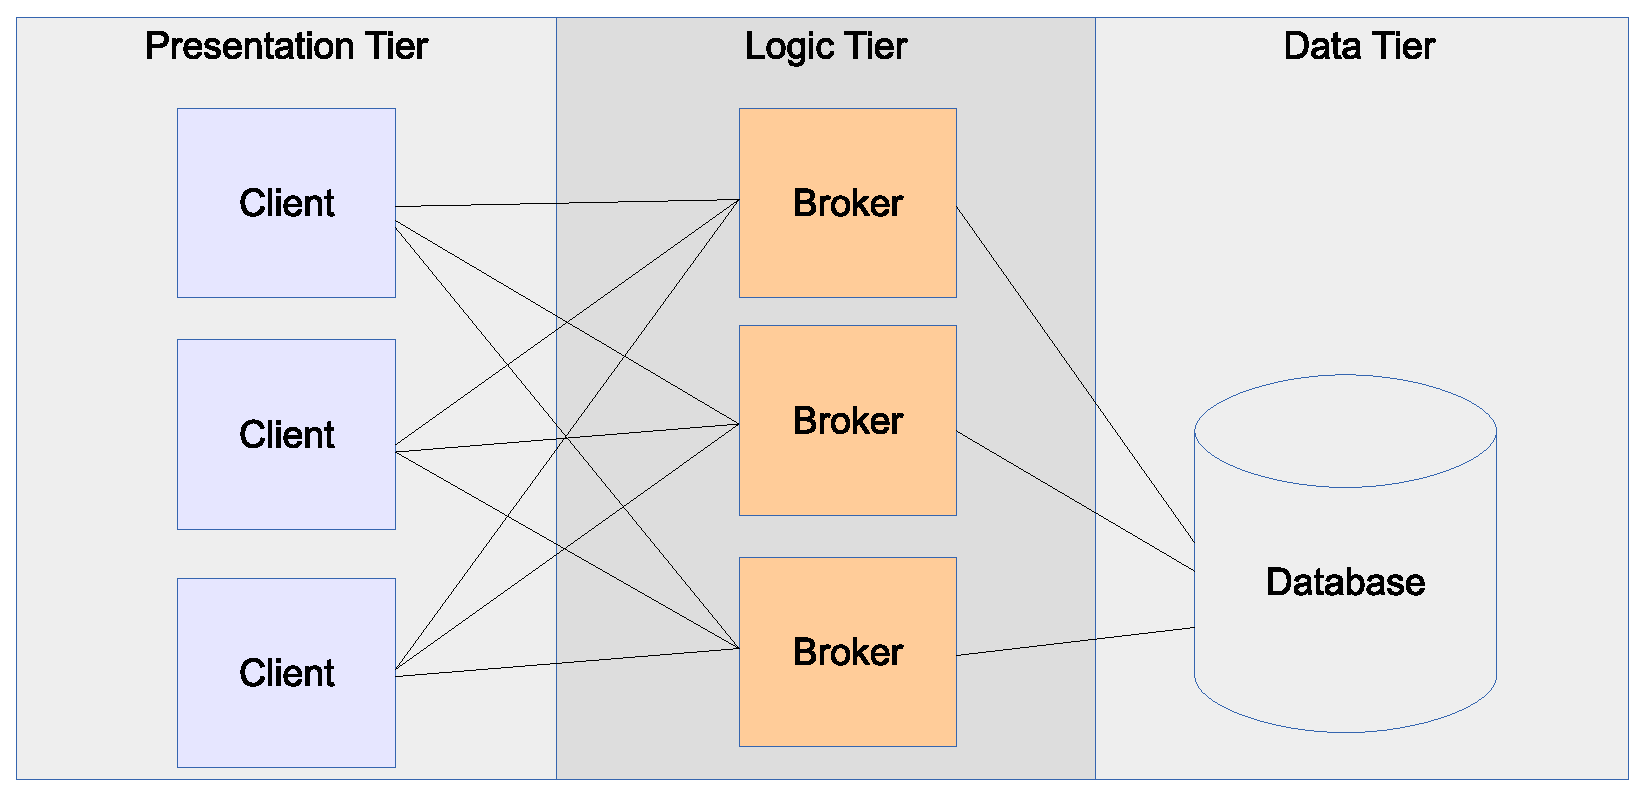
\includegraphics[scale=0.3]{../../drawings/system-overview.eps}
    
  \end{center}
  \caption{System Overview}
  \label{fig:system-overview}
\end{figure}


\end{frame}

\section{Messaging System}

\begin{frame}
\frametitle{System Overview}
\begin{itemize}
\item The messaging system utilizes a single database instance. 
\item On the logic tier multiple broker instances may be running. 
\item Each broker is responsible for certain queues.
\item Clients may ask any broker about who handles requests for a specific queue.
\item A client may connect to any number of brokers depending on which target queue it wants to send messages.
\end{itemize}
\end{frame}




\begin{frame}
\frametitle{Broker Threading}
\begin{figure}
  \begin{center}
    \includegraphics[scale=0.42]{../../drawings/broker-threading.eps}
  \end{center}
  \caption{Broker Threading}
  \label{fig:broker-threading}
\end{figure}


\end{frame}


%% \begin{frame}
%% \frametitle{Server networking}
%% \begin{itemize}
%% \item Java NIO (Reactor or Leader/Followers)
%% \end{itemize}
%% http://www.kircher-schwanninger.de/michael/publications/lf.pdf
%% \end{frame}



\section{Database}
\begin{frame}
\frametitle{Database Schema}

\begin{figure}
  \begin{center}
    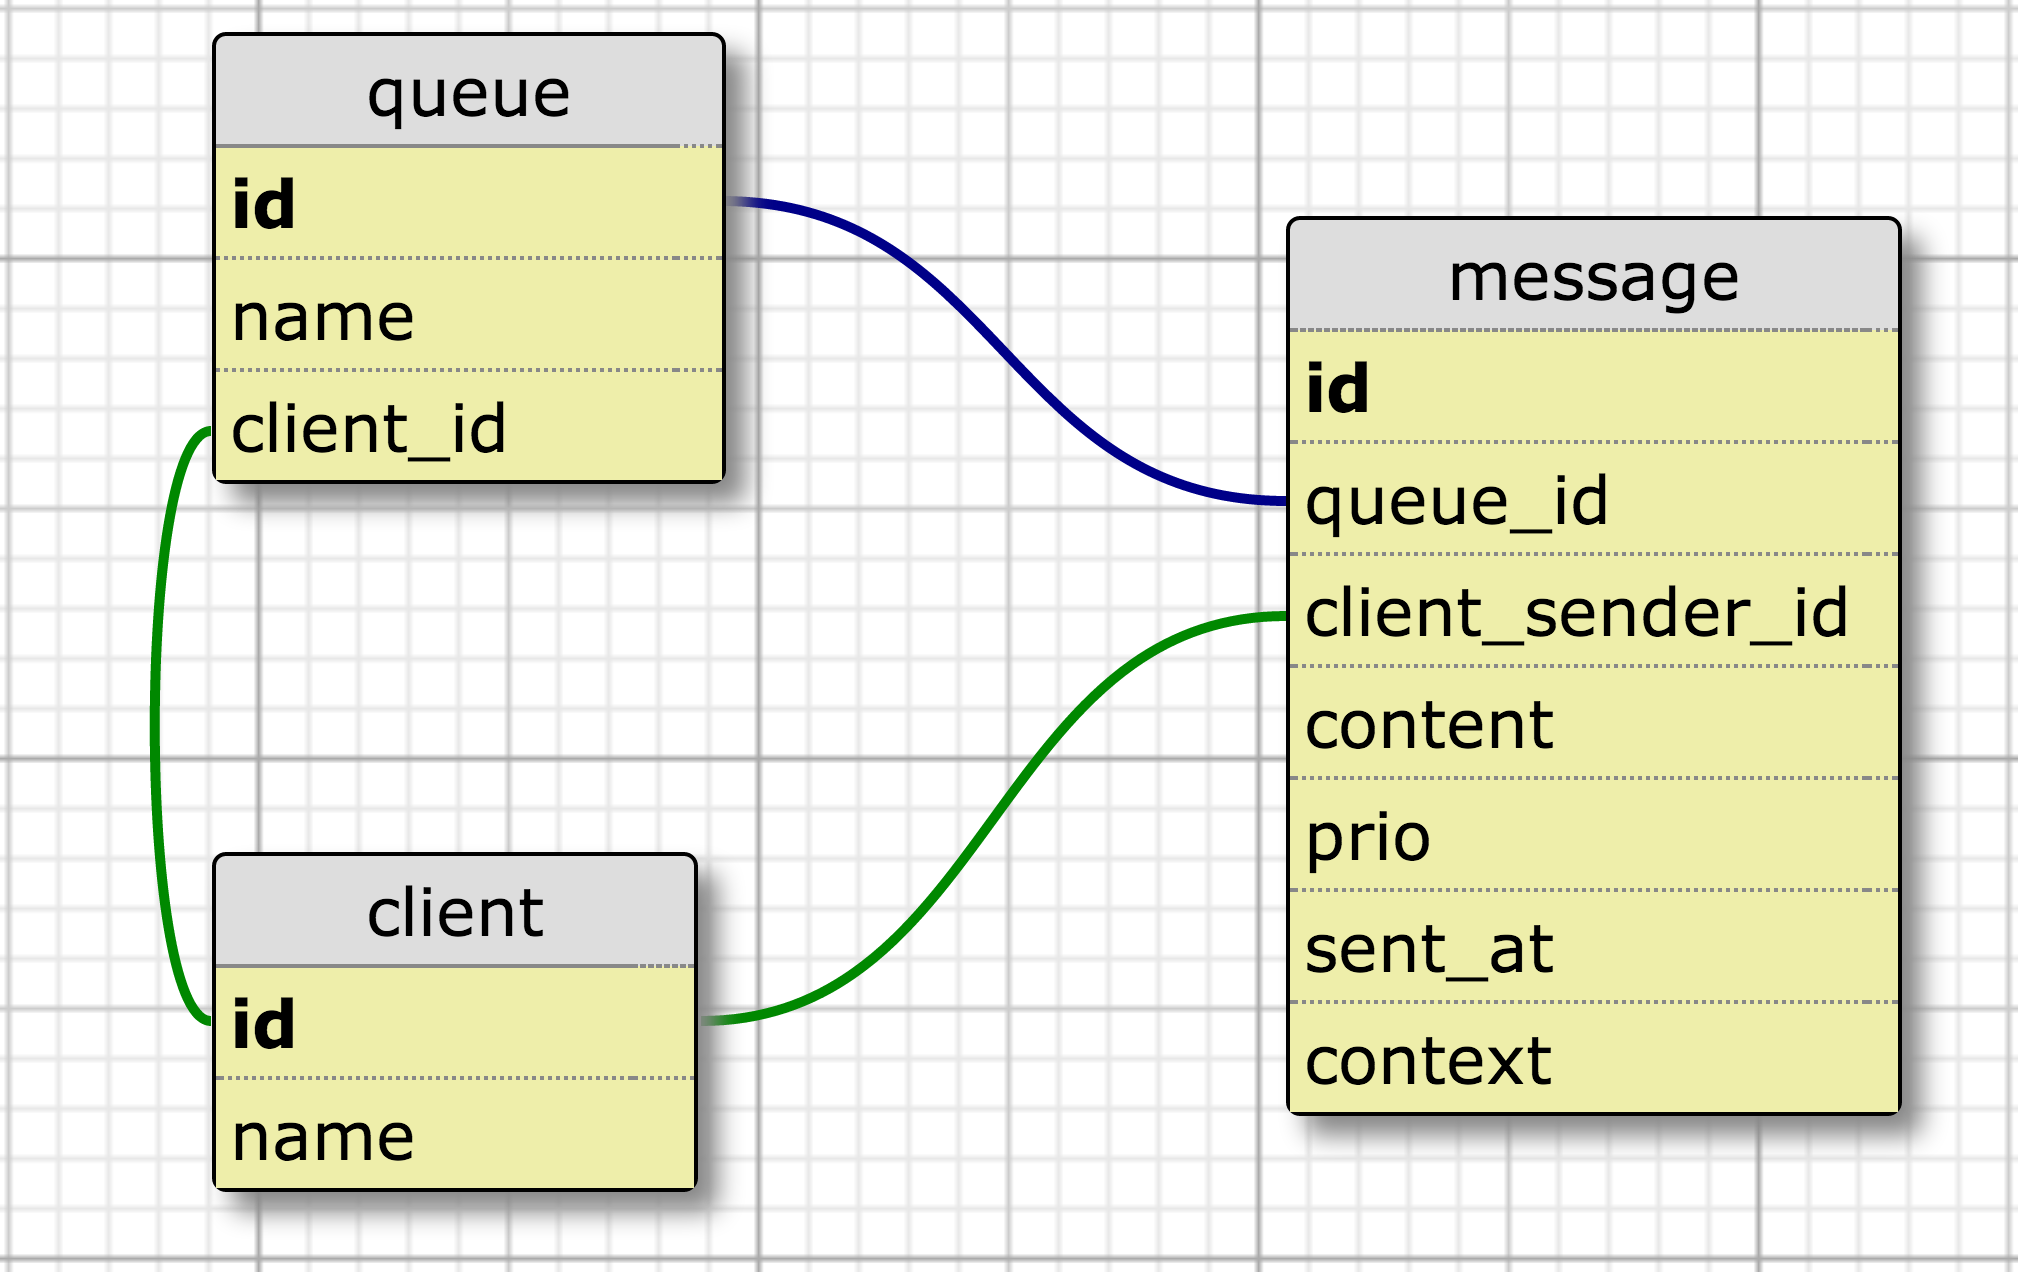
\includegraphics[scale=0.42]{../../database/db-schema.png}
  \end{center}
  \caption{Database Schema}
  \label{fig:db-schema}
\end{figure}
\end{frame}



\begin{frame}
\frametitle{Client to Broker Communication}

\begin{itemize}
\item Header: Length of the Java object in bytes.
\item Body: Serialized Java object (Request, Response).
\item Serialize POJO's and send it over the network
\item Connection: keep alive, connection pool
\item Security: no authentication, no encryption
\end{itemize}
\end{frame}



\section{Client}
\begin{frame}
\frametitle{Client}
\begin{itemize}
\item Clients may have different configurations depending on the test case currently performed.
\begin{itemize}
\item{Only send messages}
\item{Only read messages}
\item{Only do request/response}
\end{itemize}

\item Management interface in HTTP
\begin{itemize}
\item{To start/stop the current action}
\item{To collect statistics}
\end{itemize}
\item Use any Browser as Management Interface
\end{itemize}
\end{frame}





\section{Request}
\begin{frame}
\frametitle{Request}

\begin{figure}
  \begin{center}
    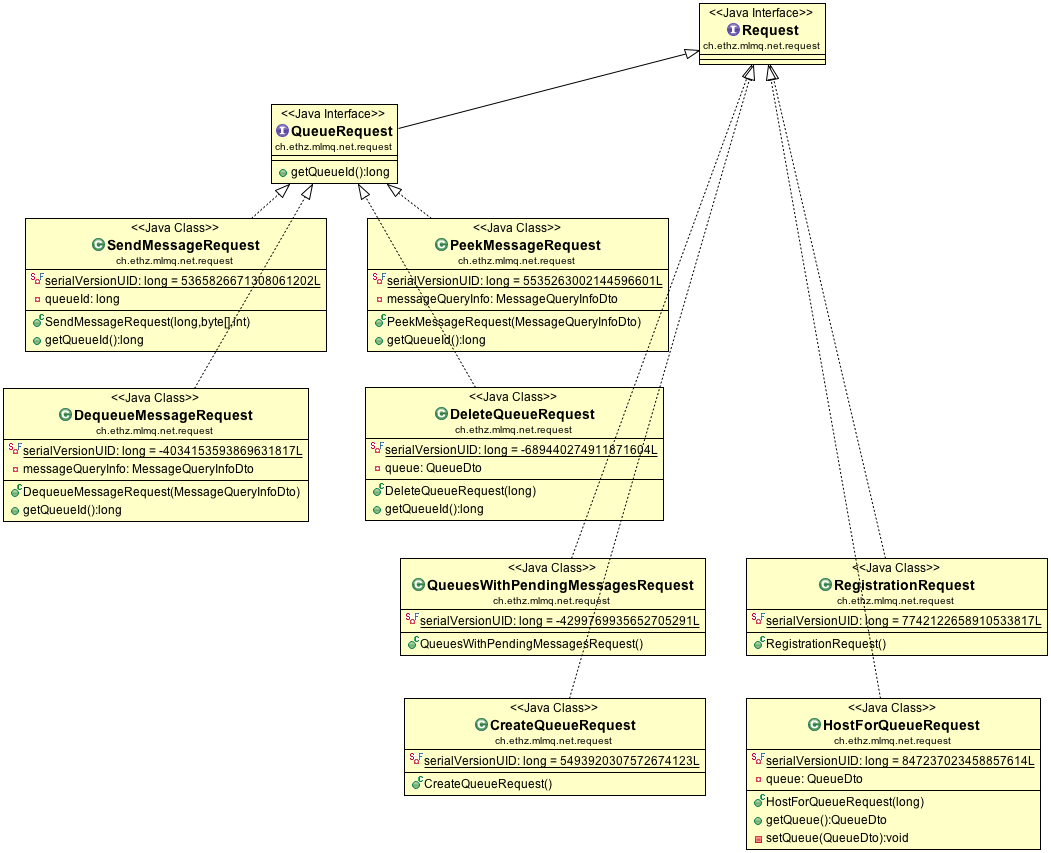
\includegraphics[scale=0.25]{../../class_diagrams/Request.png}
  \end{center}
  \caption{Request Class Diagram}
  \label{fig:db-schema}
\end{figure}

\end{frame}



\section{Response}
\begin{frame}
\frametitle{Response}

\begin{figure}
  \begin{center}
    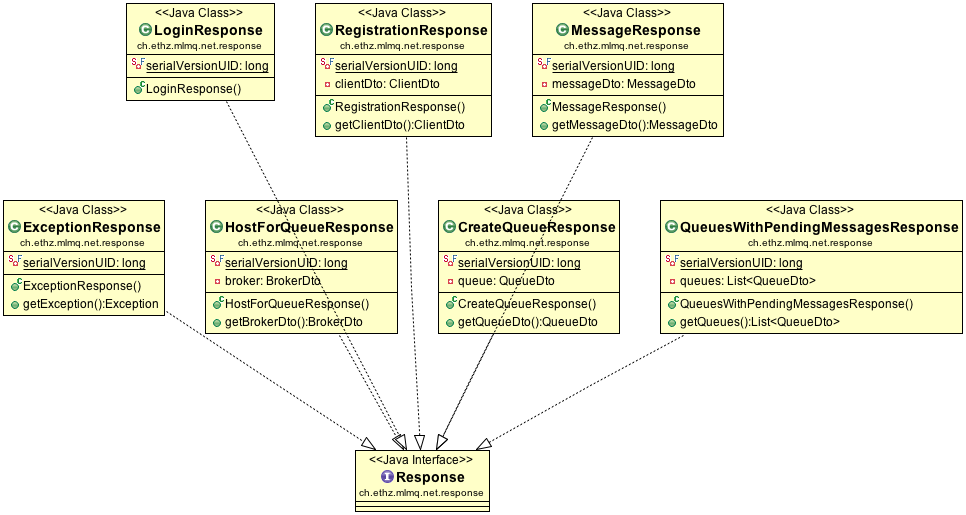
\includegraphics[scale=0.33]{../../class_diagrams/Response.png}
  \end{center}
  \caption{Response Class Diagram}
  \label{fig:db-schema}
\end{figure}

\end{frame}




\end{document}

